\documentclass[12pt]{article}          % 12-point font
\usepackage{natbib}
\usepackage{afterpage}
\usepackage{booktabs}
\usepackage{tabularx}
\usepackage[margin=1in]{geometry}
\usepackage{booktabs}
\usepackage{longtable}
\usepackage{array}
\usepackage{pdflscape}
\usepackage{listings}
\usepackage[most]{tcolorbox}

\usepackage{graphicx}
\usepackage{float}
\usepackage{tikz}
\usepackage{pgfplots}
\usepackage{adjustbox}
\usepackage{subcaption}
\usepackage[normalem]{ulem}
\usepackage[hidelinks]{hyperref}
\usepackage[capitalise, noabbrev]{cleveref}
\usetikzlibrary{positioning, arrows.meta, calc}
\newcommand{\ttl}[1]{{\sffamily\bfseries\small #1}}
\newcommand{\sub}[1]{{\sffamily\scriptsize\color{black!62} #1}}
\graphicspath{{images/}}
\usepackage[margin=1in]{geometry}      % 1-inch margins on all sides
\usepackage{setspace}
\doublespacing   

% Ragged-right fixed-width column used by the SI tables
\newcolumntype{P}[1]{>{\raggedright\arraybackslash}p{#1}}

\title{How Teams Regroup in the Seconds After a Setback}
% TODO: add affiliations and corresponding-author contact
\author{Ava Grey \and Evey Huang \and Matt Groh}
\date{}

\begin{document}
\maketitle
\begin{abstract}
The difference between a temporary setback and a downward slide often comes down to what a team does next. In high-stakes environments, a team may only have seconds to respond during the transition phases between performance episodes. However, these transition phases are too brief for surveys to capture and occur too often to hand-code at scale. How do teams respond in the seconds after a setback, and how does their response influence their subsequent performance? We study collegiate volleyball, where every rally ends in an unambiguous point, and teammates respond by huddling briefly before the next serve. Using computer vision to convert match video into players' court positions, we measure 10,362 huddles by 48 teams across 32 NCAA Division III women's matches and link each huddle to the rallies before and after it. We find that teams tend to deploy a setback-specific recovery pattern in which players huddle longer, take longer to form the huddle, and huddle closer together, and this pattern strengthens as teams experience compounding losses.  We do not find that a single huddle predicts the next rally better than chance. However, we find that teams that consistently follow the recovery pattern win more often and by more points. These results, based on computer vision-extracted microdynamics of team huddles, present preliminary evidence that reliability of a recovery routine tracks and predicts team performance.
\end{abstract}

\section{Motivation}

In high-stakes, fast-paced environments, teams often have only a brief moment to respond to a setback, and how they respond can shape whether the setback’s effect on future performance compounds or dissipates. For example, a surgical team may quickly huddle after one member makes an error to discuss how to complete the operation safely. These brief moments when teams step away from performance to huddle and evaluate what happened and plan for next steps are called transition phases \citep{marks2001temporally}.  Organizational scholars have discovered that teams are more likely to bounce back from the setback when they allow members to safely discuss errors \citep{edmondson1999}, draw on shared resources \citep{stoverink2020}, and surface potential threats \citep{goldenhar2013huddling} during these phases.  But if they treat setbacks as threats, they start to constrict attention and centralize
control; the original setback could compound \citep{staw1981}. 

% Teams in which members feel safe to discuss errors engage in more learning behavior \citep{edmondson1999}, and resilient teams draw on shared resources to bounce back from setbacks together \citep{stoverink2020}. Teams evaluate what happened and plan what comes next in the transition phase between performance episodes \citep{marks2001temporally}, but they can also treat setbacks as threats, constricting attention and centralizing control in ways that compound the original setback \citep{staw1981}. Huddles are one way teams use these transition phases. Hospitals hold safety huddles to surface threats before they cause harm \citep{goldenhar2013huddling}, and effective teams step away from the task for brief huddles to reallocate their remaining time \citep{fisher2024clock}.

But we still know little about teams' behavior during these transition phases. Surveys capture teams' perceptions of what happens but not what they actually do \citep{WallerandKaplan}. Retrospective analysis captures whether a team recovered from a setback but not how it did so. Human annotators can code some of these interactions \citep{kraus2010, durdubas2021}, but hand-coding is too expensive to scale and can miss phases that last only seconds. Recent studies have started to use computational methods. For example, \cite{Serpell2023} used GPS to track rugby players' huddling behavior across 100 professional games but found no relationship with performance. Finding defensible patterns between team recovery and performance requires measurement that scales across thousands of moments and links each one to the setback that preceded it.

%Current literature is missing systematic evidence about what happens during these huddles after preceding setbacks. Transition phases are moments that can tell us a lot about teams, and while they recur many times within a single performance, they often last only seconds. Surveys merely capture team members’ perceptions, and retrospective outcome analysis cannot measure what a team actually does during the recovery moments  \citep{WallerandKaplan}. Behavioral coding, while it can capture some interactions, struggles to reach a scale that can identify defensible patterns. GPS tracking of player clustering during stoppages across 100 professional rugby games found no link to match performance \citep{Serpell2023}. Linking regrouping to performance requires both scale and resolution to a single setback. 

We propose to use collegiate volleyball to study team behavior in transition phases because setbacks are frequent and unambiguous, and each one is followed by a brief regrouping moment. Every rally yields a win for one team and a loss for the other; each team averages 87 lost points per game, and in the seconds before the next rally teammates often huddle and then break to their positions to continue the game. We treat this huddle as the team’s regrouping: a bounded, observable transition phase whose timing and shape we can measure. Because the rules control serving, rotation, and timeouts, we can separate regrouping a team chooses from interactions the rules require. Following past work that uses sports as a model system for organizational science \citep{dai2018quitting, day2012sporting, fonti2023sports, humphrey2014microdynamics}, we ask: How do volleyball teams regroup in the seconds after a setback, and does how they regroup relate to their performance?

\section{Core Scientific Contribution}
We develop an AI pipeline that takes full volleyball games and outputs temporal and spatial data from huddle moments. We characterize three properties of a team’s huddle interaction: time to converge, duration while in the huddle, and closeness during the huddle. We applied our pipeline to thousands of huddles, yielding repeated measurements that give us enough data to identify patterns within and across teams. Our framework enables us to measure team dynamics as an observational, behavioral measure \citep{kozlowskichao2018}. 

We found that teams respond to setbacks with a clear regrouping pattern that intensifies as setbacks compound. Consistent post-point huddle rituals that follow the pattern of taking longer to come together, staying together longer, and coming together closer are positively related to team win percentage, while no single huddle predicts the outcome of the next rally. The remaining question is whether these regrouping patterns contribute to recovery, measure other team capabilities, or stem from game-related situations.

Through measuring regrouping directly, we can examine these questions empirically and make three contributions. First, we place a setback response in the transition phase, where team process theory argues for it, and offer a way to distinguish resilient coordination from threat-induced cohesion. Second, we distinguish the regrouping pattern from its consistency across setbacks, echoing work on the relationship between regrouping patterns and variable performance \citep{feldman2003}. Last, we introduce a low-cost AI pipeline that takes full game footage and turns it into measurable transition episodes at \$0.06 per huddle, creating a new empirical measure for studying team dynamics \citep{kozlowskichao2018}. Together, our contributions create a framework for investigating how and when teams regroup following repeated setbacks. 

\section{What we have done}
\subsection{Data and Pipeline}
We collected 32 Division III women's volleyball games from YouTube. Division III games offer optimal camera angles that capture huddles from both teams. The 32 games span the years 2019 through 2025 and include 48 unique teams and 39 unique schools, yielding 10,362 huddles for our analysis. 

We implemented an AI-powered pipeline to process raw huddle data as team-level behavioral interactions. We used an MLLM to identify huddle moments during games and an AI computer vision model to track each team member throughout a huddle episode. With this information, we calculated team-level properties that describe the huddle as a whole. We identify three spatiotemporal features of huddles: \textit{latency}, \textit{closeness}, and \textit{duration} (see Appendix A for further details). Figure~\ref{fig:pipeline} in the Appendix shows how we transform video footage into huddle-level statistics that we combine with performance-based metrics. 

After obtaining three descriptive statistics that capture the entire huddle interaction, we mapped these features to previous and future point outcomes. After standardizing the features within games, we examined how teams deviate from their normal rituals, how teams differ in recovery patterns, and how these patterns relate to a team's success. We regressed each standardized feature on the preceding point outcome or streak state with game fixed effects and huddle-clustered standard errors. 



\subsection{Preliminary Results}
Our analysis asks three main questions: do teams exhibit recovery behaviors in time-limited moments, how do recovery patterns change during compounded losses, and how important are short recovery moments for future success? Across 10,362 huddles and 32 games, teams deploy a setback-specific pattern that strengthens as teams experience compounded losses and relates to future success.

\subsubsection{Teams deploy setback-specific huddle rituals}

After losing a point, teams come together more slowly and stay together longer. Specifically, teams stay together 0.291 SD (p $<$ 0.001) longer and come together 0.544 SD (p $<$ 0.001) slower. Teams do not huddle any closer after losses than after wins. The huddle interaction features carry information on the outcome of the last point. However, they carry no predictive power for the immediate next point. Regressing on all three features to predict whether a team will win or lose the next point, given how they interacted in the prior huddle, is no better than random chance (AUC = 0.5). 

During compounded losses, teams follow a clear huddling pattern that strengthens monotonically as the losing streak worsens. For example, after a single loss, teams huddle longer and take longer to come together as losses continue. These behaviors become more extreme as teams experience more losses. Additionally, after teams lose two points in a row, they statistically huddle closer. As teams fall deeper in losing streaks, their huddle behaviors more closely follow the pattern of staying together longer, taking longer to come together, and huddling closer together (as seen in Figure 1a). The three huddle properties together predict whether a team is in a losing streak far better than chance (AUC = 0.715).

\subsubsection{Setback response relates to overall performance}

We introduce a team-level measure, \textit{recovery-routine consistency}, that pairs how strongly a team follows the dominant recovery pattern during a losing streak (coming together slower, staying together longer, and huddling closer) with how often it follows it.

Within games, the team that followed the recovery pattern more consistently won 72\% of the time (23 of 32 games, $p = 0.020$; Figure 1b). Among the 32 winners, the 23 with higher consistency won by an average of 13.7 points, compared with 9.8 points for the 9 with lower consistency. Across teams, recovery-routine consistency also correlates positively with team win percentage ($r = 0.361$, $p = 0.012$; Figure 1c).

As a robustness check, teams with higher and lower recovery-routine consistency experience a similar number of losing streaks of similar lengths (mean length 2.83 vs. 2.85; $p > 0.1$), so consistency is not driven by how many losing streaks a team experiences. Our findings also do not differ between early-game and late-game situations, suggesting huddle behavior is not just an outcome of the game-specific situation.

\begin{figure}[H]
    \centering
    \captionsetup[subfigure]{skip=2pt}% less space between each image and its subcaption
    \def\figscale{0.85}% <- lower = shorter figure
    \begin{subfigure}[t]{\figscale\dimexpr0.77\linewidth\relax}
        \centering
        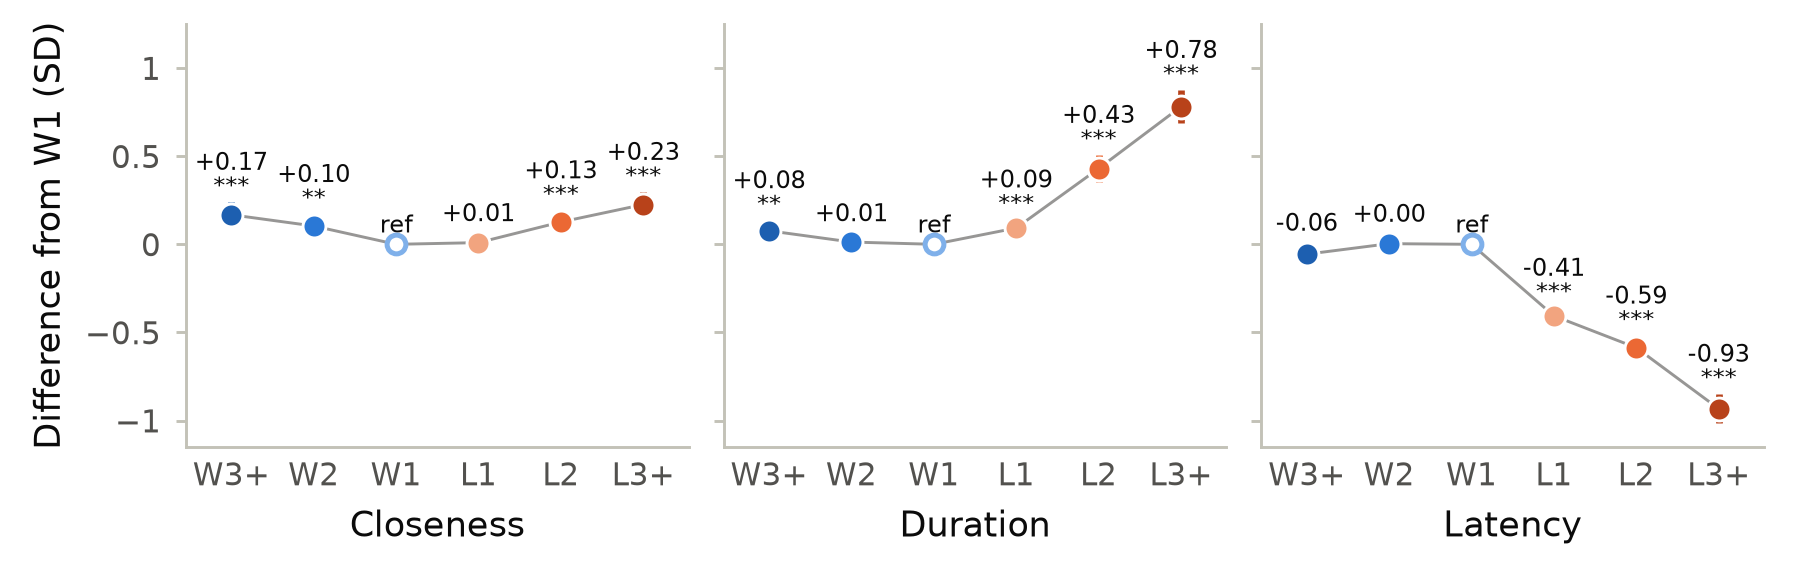
\includegraphics[width=\linewidth]{images/run_state_profile.png}
        \caption{Huddle closeness, duration, and latency by momentum state, relative to a single point just won (W1). Effects in within-game SD. Features are oriented so that higher values indicate tighter, longer, and faster huddles.}
        \label{fig:run_state}
    \end{subfigure}

    \vspace{0.2em}
    \begin{subfigure}[t]{\figscale\dimexpr0.37\linewidth\relax}
        \centering
        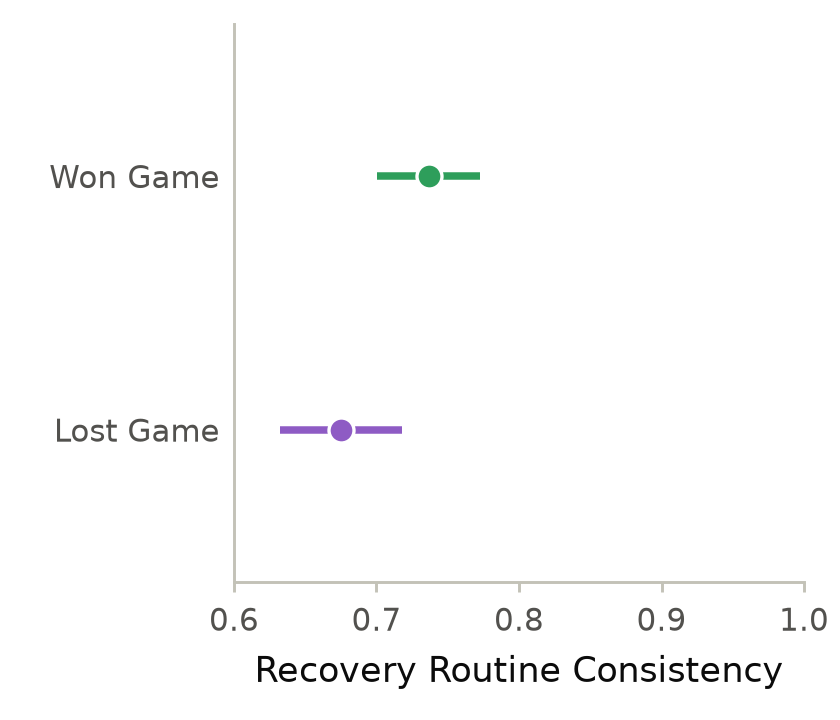
\includegraphics[width=\linewidth]{images/recovery_routine_consistency_OLS.png}
        \caption{Recovery consistency for teams that won versus lost the game (mean, 95\% CI).}
        \label{fig:won_lost}
    \end{subfigure}
    \hspace{\figscale\dimexpr0.03\linewidth\relax}
    \begin{subfigure}[t]{\figscale\dimexpr0.37\linewidth\relax}
        \centering
        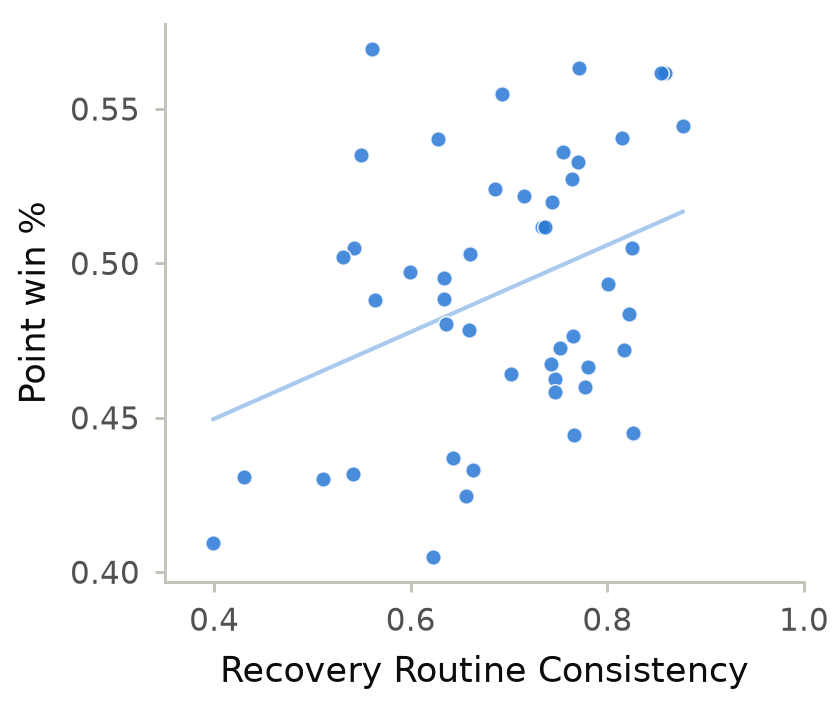
\includegraphics[width=\linewidth]{images/auc_vs_winpct.png}
        \caption{Team-level recovery consistency versus point-win percentage.}
        \label{fig:teams}
    \end{subfigure}
    \vspace{-0.3em}
    \caption{Huddle behavior after setbacks and its relationship to winning.}
    \label{fig:combined}
\end{figure}


\section{Risks}
We acknowledge four potential risks of our proposed work. First, our geometric features are not resilience or emotional regulation themselves, and we do not know the exact recovery mechanism a team uses. For example, we cannot say that a team coming together more quickly shows a higher level of shared resilience. Rather, these are observable behaviors that provide insight into these latent processes. Second, our analysis is associational, so we cannot currently say that huddling causes recovery. Third, using sports as our domain introduces potential noise into our performance metrics. While scoring a point in volleyball is inherently team-dependent \citep{EomSchutz}, considerable randomness affects whether an action succeeds or fails. A single-point outcome may not cleanly measure whether a team recovers from a setback. Lastly, volleyball creates clear action-recovery-action episodes that most other domains do not define as cleanly. So, while our work builds the foundation for the microdynamics of team recovery, extending it to domains without clear, observable recovery moments will require further generalization. 



\section{Proposed Future Work}
First, to better understand \textit{when} teams initiate coordination and recovery, we need to extend our analysis beyond simple wins and losses. Not all losses carry the same degree of failure. Recent literature asks this as an open question: which characteristics of adversity matter for team recovery \citep{bisbey2025towards}. Losses that occur unexpectedly–a higher-ranked team surprisingly losing to a lower-ranked team–could result in different recovery behavior. For example, \citet{dai2018quitting} found that individuals who are expected to win but fall behind are more likely to quit than underdogs. More game-level data would let us test these questions.

Huddle geometric variables are a good starting point, but recovery can involve many more variables. Facial expressions, touch frequency, body language, gestures, and the words teammates say can offer insight into how teams process setbacks and respond. Measuring whether certain individuals dominate the recovery process, like standing in the middle of a huddle, would show whether this behavior affects individual and team performance.

Because terminal sports metrics tend to be very noisy \citep{berger2011losing}, more analysis is needed on when recovery works for a team and when it doesn’t. While we found that immediate next-point success is null, we found that game-level performance was significant. Additional questions remain about aggregate-level metrics, like over an entire season, or through mediating variables. There exists a strong opportunity to study what recovery leads to, since it is often measured as an outcome itself rather than a predictor \citep{kirkman2026team}. Outcomes to explore could include streak length; coordination quality; teammate re-involvement; or variation in performance under accumulated adversity.

We believe our proposed approach of measuring transition-phase behavior directly from existing video could change how organizational science studies team dynamics by making the time between setbacks and renewed action observable temporally and at scale. Rather than relying on surveys that offer only static snapshots, researchers could measure recovery as a series of action-recovery-action episodes at a team level. With careful consideration of context, our computer vision-based team process measurement pipeline could be extended into other fast-paced domains like medical teams, military teams, flight crews, and emergency response.


\clearpage
\bibliographystyle{apalike}
\bibliography{references}

\clearpage
\appendix
\section*{Supplementary Information}
\section{Data collection and huddle segmentation}
% ===== PIPELINE FIGURE (v3: three stacked panels) — paste where the figure should go =====
% Preamble needs:  \usepackage{tikz} \usepackage{graphicx} \usepackage{adjustbox} \usepackage{float}
%                  \usetikzlibrary{arrows.meta, positioning, calc, decorations.pathreplacing}
% Real numbers come from figstats.tex + data/*.dat (written by make_figure_data.py).
% Without them the figure still compiles, with XX / placeholder curves.
% (tikz libraries are loaded in the preamble)

% ---------------- numbers shown in the figure ----------------
\IfFileExists{figstats.tex}{\input{figstats.tex}}{}
\providecommand{\figNGames}{32}      \providecommand{\figNTeams}{48}
\providecommand{\figYears}{2019--2025}
\providecommand{\figNClips}{5{,}571} \providecommand{\figMeanClip}{XX}
\providecommand{\figCost}{\$0.06}
\providecommand{\figNRaw}{11{,}142}  \providecommand{\figNKept}{10{,}362}
% KDE panels
\providecommand{\figMedClose}{7}  \providecommand{\figXminClose}{2} \providecommand{\figXmaxClose}{14} \providecommand{\figTicksClose}{4,8,12}
\providecommand{\figMedDur}{4}    \providecommand{\figXminDur}{0}   \providecommand{\figXmaxDur}{12}   \providecommand{\figTicksDur}{0,5,10}
\providecommand{\figMedLat}{3}    \providecommand{\figXminLat}{0}   \providecommand{\figXmaxLat}{10}   \providecommand{\figTicksLat}{0,4,8}
% example huddle in panel (c): times in s, spreads in ft
\providecommand{\exXmax}{10}  \providecommand{\exYmax}{12}
\providecommand{\exXticks}{0,5,10} \providecommand{\exYticks}{0,5,10}
\providecommand{\exThr}{5.8}                       % "tight" cutoff
\providecommand{\exTin}{3.6}  \providecommand{\exTout}{7.3}   % enters / leaves tight zone
\providecommand{\exTmin}{5.3} \providecommand{\exSmin}{3.7}   % tightest moment
\providecommand{\exSzero}{10.8}                      % spread when the point ends

% ---------------- image helpers ----------------
\providecommand{\vbimg}[2]{%
  \IfFileExists{images/#2}%
    {\includegraphics[width=#1]{images/#2}}%
    {\tikz\node[draw=black!30, fill=black!5, minimum width=#1,
       minimum height=0.6*#1, font=\tiny\ttfamily, text=black!50]{\edef\vbtmp{#2}\detokenize\expandafter{\vbtmp}};}%
}
\ifdefined\vbbox\else\newsavebox{\vbbox}\fi
\providecommand{\vbimgcr}[4]{% height, crop fraction per side, file, corner radius
  \IfFileExists{images/#3}%
    {\sbox{\vbbox}{\adjustbox{trim={#2\width} 0pt {#2\width} 0pt, clip, height=#1}%
       {\includegraphics{images/#3}}}%
     \tikz{\clip[rounded corners=#4] (0,0) rectangle (\wd\vbbox,{\ht\vbbox+\dp\vbbox});
           \node[anchor=south west, inner sep=0pt] at (0,0) {\usebox{\vbbox}};}}%
    {\tikz\node[draw=black!30, fill=black!5, rounded corners=#4, minimum width=1.42*#1,
       minimum height=#1, font=\tiny\ttfamily, text=black!50]{\detokenize{#3}};}%
}

% ---------------- square images for the four moments ----------------
% \vbcover: scale until the image fills the square, then trim equal amounts from both
%           edges (keeps the centre, no stretching).
% \vbfit:   show the whole image at its true shape, with white padding in the square.
% Pick one in \vbsqimg below.
\ifdefined\vbsqbox\else\newsavebox{\vbsqbox}\fi
\ifdefined\vbtx\else\newlength{\vbtx}\newlength{\vbty}\fi
\providecommand{\vbmissing}[1]{{\tiny\ttfamily\color{black!50}\edef\vbtmp{#1}\detokenize\expandafter{\vbtmp}}}
\providecommand{\vbcover}[2]{%
  \IfFileExists{images/#2}{%
    \sbox{\vbsqbox}{\includegraphics[height=#1]{images/#2}}%
    \ifdim\wd\vbsqbox<#1\relax\sbox{\vbsqbox}{\includegraphics[width=#1]{images/#2}}\fi
    \setlength{\vbtx}{\dimexpr(\wd\vbsqbox-#1)/2\relax}%
    \setlength{\vbty}{\dimexpr(\ht\vbsqbox+\dp\vbsqbox-#1)/2\relax}%
    \clipbox{{\vbtx} {\vbty} {\vbtx} {\vbty}}{\usebox{\vbsqbox}}%
  }{\vbmissing{#2}}%
}
\providecommand{\vbfit}[2]{%
  \IfFileExists{images/#2}%
    {\includegraphics[width=#1, height=#1, keepaspectratio]{images/#2}}%
    {\vbmissing{#2}}%
}
\providecommand{\vbsqimg}{\vbcover}   % <- change to \vbfit for whole image + padding

\definecolor{accent}{RGB}{150,120,210}
\definecolor{teamA}{RGB}{226,96,64}
\definecolor{curvecol}{RGB}{214,48,49}   % match the circle colour in your BEV images
\definecolor{teamB}{RGB}{70,110,210}

% Placed exactly here ([H]). Put \clearpage BEFORE the section header, not here.
\begin{figure}[H]
\centering
\adjustbox{max width=\textwidth, max totalheight=0.5\textheight}{%
\begin{tikzpicture}[
    >={Stealth[length=2.6mm, width=2mm]},
    flow/.style    ={->, line width=0.9pt, black!80},
    dflow/.style   ={flow, dashed},
    ptitle/.style  ={font=\Large\bfseries, anchor=north west},
    stage/.style   ={rectangle, rounded corners=10pt, fill=black!6, draw=none},
    clipfile/.style={rectangle, rounded corners=4pt, fill=accent!15, draw=accent,
                     line width=0.7pt, minimum width=3.4cm, minimum height=0.8cm,
                     font=\ttfamily\Large\bfseries},
    lab/.style     ={font=\Large, text=black!85, align=center},
    stat/.style    ={font=\large, text=black!55, align=center},
    divider/.style ={black!25, line width=1pt},
    handoff/.style ={->, accent!85!black, line width=1.6pt, rounded corners=10pt},
    hchip/.style   ={rectangle, rounded corners=5pt, fill=white, draw=accent!85!black,
                     line width=1pt, inner sep=5pt, font=\large,
                     text=accent!60!black, align=center},
]
\def\W{30}   % canvas width (cm)
%
% =====================================================================
% (a) FINDING HUDDLES
% =====================================================================
\node[ptitle] (ta) at (0,0) {(a) Finding the huddles {\mdseries\color{black!50} (in each of the \figNGames\ games)}};
%
% pile of game videos
\foreach \dx/\dy/\f/\nm in {-0.35/0.35/berry_emory.png/pileA, 0/0/laverne_southwestern.png/pileB, 0.35/-0.35/hope_calvin.png/pileC}
  \node[fill=white, draw=black!35, inner sep=1.5pt] (\nm) at ({3.6+\dx},{-3.2+\dy}) {\vbimg{4.8cm}{\f}};
\node[lab, font=\Large\bfseries, anchor=north] (games) at ($(pileC.south -| 3.6,0)+(0,-0.3)$) {\figNGames\ games};
\node[stat, below=0pt of games] {D-III women's volleyball\\\figYears\ $\cdot$ \figNTeams\ teams};
%
% segmentation
\node[stage, minimum width=11.0cm, minimum height=4.6cm] (seg) at (14.85,-3.5) {};
\node[lab, font=\Large\bfseries] at ($(seg.north)+(0,-0.5)$) {Huddle clipping};
\node (gem) at ($(seg.center)+(-2.8,0.15)$) {\vbimg{1.5cm}{gemini.png}};
\node (hum) at ($(seg.center)+( 2.8,0.15)$) {\vbimg{1.5cm}{user.png}};
\node[font=\LARGE\bfseries] at ($(gem)!0.5!(hum)$) {+};
\node[below=3pt of gem, font=\ttfamily\normalsize, align=center] {gemini-3.1\\-pro-preview};
\node[below=3pt of hum, font=\large, text=black!75, align=center] {person checks\\\& fixes};
\node[stat, below=4pt of seg] {\figCost\ per huddle};
\draw[flow] ($(pileC.east |- seg.west)+(0.3,0)$) -- ($(seg.west)+(-0.25,0)$);
%
% clips
\def\cx{25.6}
\node[stat, align=center] at (\cx,-0.95) {one game $\to$ up to 5 sets,\\$\sim$45 huddle clips per set};
\node[clipfile] (c1) at (\cx,-2.0) {H1\_S1.mp4};
\node[clipfile] (c2) at (\cx,-3.1) {H2\_S1.mp4};
\foreach \dy in {-0.2,0,0.2} \fill[black!70] (\cx,{-4.05+\dy}) circle (1.6pt);
\node[clipfile] (c4) at (\cx,-5.0) {H23\_S5.mp4};
\coordinate (fan) at ($(seg.east)+(0.3,0)$);
\foreach \c in {c1,c2,c4} \draw[flow] (fan) -- ($(\c.west)+(-0.15,0)$);
\draw[dflow] (fan) -- (\cx-1.9,-4.05);
%
%
%
% =====================================================================
% (b) LOCATING PLAYERS
% =====================================================================
\node[ptitle] (tb) at (0,-7.7) {(b) Locating the players {\mdseries\color{black!50} (in each of the \figNClips\ clips)}};
\def\by{-12.25}   % vertical centre of panel (b) content
%
% FIX 1: photos spread apart so "homography" fits between them
\node[inner sep=0pt] (courtimg) at (3.6,\by) {\vbimgcr{5.0cm}{0.10}{white_court.png}{12pt}};
\node[lab, below=5pt of courtimg] {\textbf{1.} find the court lines};
\node[inner sep=0pt] (playerimg) at (13.9,\by) {\vbimgcr{5.0cm}{0.10}{player_track.png}{12pt}};
\node[lab, below=5pt of playerimg] {\textbf{2.} find every player};
\draw[flow] ($(courtimg.east)+(0.2,0)$) -- ($(playerimg.west)+(-0.2,0)$)
     node[midway, above, font=\large, text=black!55] {homography};
%
% top-down court map (18 m x 9 m)
\def\cs{0.5556}
\coordinate (mapSW) at (19.6,{\by-2.5});
\begin{scope}[shift={(mapSW)}, x=\cs cm, y=\cs cm]
  \fill[black!4] (0,0) rectangle (18,9);
  \draw[black!45, line width=0.7pt] (0,0) rectangle (18,9);
  \draw[black!40, line width=0.5pt] (6,0) -- (6,9) (12,0) -- (12,9);
  \draw[black!80, line width=1.8pt] (9,-0.5) -- (9,9.5);
  % one frame, both teams, court coordinates in metres
  \foreach \px/\py in {8.15/0.41, 8.11/2.41, 6.54/8.09, 5.7/1.56, 4.47/6.22, 2.18/4.18}
    \fill[teamA] (\px,\py) circle (3pt);
  \draw[teamA, line width=1.1pt] (6.25,4.02) circle (4.08);
  \foreach \px/\py in {12.26/2.25, 9.67/2.43, 10.47/3.74, 9.91/5.9, 13.03/6.67}
    \fill[teamB] (\px,\py) circle (3pt);
  \draw[teamB, line width=1.1pt] (11.35,4.55) circle (2.71);
  \coordinate (mapNE) at (18,9);
\end{scope}
\node[inner sep=0pt, minimum width={18*\cs cm}, minimum height={9*\cs cm}, anchor=south west] (map) at (mapSW) {};
\node[lab, below=5pt of map] (maplbl) {\textbf{3.} map every player onto the court, frame by frame (ft)};
\draw[flow] ($(playerimg.east)+(0.2,0)$) -- ($(map.west)+(-0.2,0)$);
%
%
%
% hand-off (a) -> (b): every clip runs through the same steps
\def\laneA{-8.95}
\draw[handoff] ($(c4.south)+(0,-0.15)$) -- (\cx,\laneA) -- (courtimg.north |- 0,\laneA)
     -- ($(courtimg.north)+(0,0.15)$);
\node[hchip] at ($(courtimg.north |- 0,\laneA)!0.5!(\cx,\laneA)$) {all \figNClips\ clips from the \figNGames\ games};
%
% =====================================================================
% (c) MEASURING EACH HUDDLE
% =====================================================================
\node[ptitle] (tc) at (0,-16.4) {(c) Measuring each huddle {\mdseries\color{black!50} (one example, then all \figNKept)}};
%
\begin{scope}[yshift=-1.9cm]
%
% ---- filmstrip: four moments, game video on top, bird's-eye view below ----
\def\sq{2.2cm}          % side of each square frame
\def\sqin{2.2cm}                   % size of the image inside the square
\tikzset{sqframe/.style={rectangle, inner sep=0pt, minimum width=\sq, minimum height=\sq,
          draw=black!30, line width=0.5pt, rounded corners=3pt, fill=white}}
\def\fytop{-17.68}      % top of the video images
% images: images/moment1_video.png, images/moment1_bev.png, ... moment4
% FIX 2: frames 3.7 cm apart (was 3.5) and labels at \large (was \Large)
\foreach \nm/\fs/\x/\word/\t in {fA/moment1/2.6/point ends/0, fB/moment2/6.3/huddle forms/\exTin,
                             fC/moment3/10.0/tightest/\exTmin, fD/moment4/13.7/breaks up/\exTout} {
  \node[sqframe, anchor=north] (\nm vid) at (\x,\fytop)
       {\vbsqimg{\sqin}{\fs_video.png}};
  \node[sqframe, anchor=north] (\nm bev) at ($(\nm vid.south)+(0,-0.15)$)
       {\vbsqimg{\sqin}{\fs_bev.png}};
  \coordinate (\nm) at (\nm bev.south);
  \node[lab, anchor=south, font=\large] at ($(\nm vid.north)+(0,0.1)$)
       {\textbf{\word}\\[-1pt]{\large $t=\t$\,s}};
}
\node[font=\large, text=black!60, rotate=90, anchor=south] at ($(fAvid.west)+(-0.1,0)$) {video};
\node[font=\large, text=black!60, rotate=90, anchor=south] at ($(fAbev.west)+(-0.1,0)$) {bird's-eye};
%
% ---- spread over time for that huddle ----
\pgfmathsetmacro{\xu}{11.6/\exXmax}   % cm per second
\pgfmathsetmacro{\yu}{3.6/\exYmax}    % cm per foot
\begin{scope}[shift={(2.2,-26.63)}, x=\xu cm, y=\yu cm]
  % duration: time spent below the cutoff
  \fill[accent!16] (\exTin,0) rectangle (\exTout,\exYmax);
  % axes, ticks, labels
  \draw[black!60, line width=0.7pt, -{Stealth[length=1.8mm]}] (0,0) -- ({1.04*\exXmax},0);
  \draw[black!60, line width=0.7pt, -{Stealth[length=1.8mm]}] (0,0) -- (0,{1.08*\exYmax});
  \foreach \tk in \exXticks
    \draw[black!60, line width=0.6pt] (\tk,0) -- ++(0,-4pt)
         node[below, font=\large, text=black!70] {\tk};
  \foreach \tk in \exYticks
    \draw[black!60, line width=0.6pt] (0,\tk) -- ++(-4pt,0)
         node[left, font=\large, text=black!70] {\tk};
  \node[font=\Large, text=black!80] at ({0.5*\exXmax},0) [yshift=-1.05cm] {time since the point ended (s)};
  \node[font=\Large, text=black!80, rotate=90] at (0,{0.5*\exYmax}) [yshift=1.05cm] {enclosing circle (ft)};
  % duration
  \draw[accent!80!black, line width=1.1pt, {Stealth[length=2mm]}-{Stealth[length=2mm]}]
       (\exTin,{0.93*\exYmax}) -- (\exTout,{0.93*\exYmax})
       node[midway, above, font=\Large\bfseries, text=accent!70!black] {duration};
  % the curve (real huddle from data/example_huddle.dat if present)
  \IfFileExists{data/example_huddle.dat}%
    {\draw[curvecol, line width=1.6pt, line join=round] plot file {data/example_huddle.dat};}%
    {\draw[curvecol, line width=1.6pt] plot[smooth, tension=0.6] coordinates
       {(0,10.8) (1,10.1) (2,8.6) (3,6.8) (3.8,5.4) (4.6,4.3) (5.3,3.7) (6.1,4.0)
        (6.9,5.0) (7.6,6.5) (8.5,8.4) (9.5,9.9)};}
  % latency: from the point ending to the tightest moment
  \draw[accent!80!black, line width=1.4pt] (0,{0.08*\exYmax}) -- (\exTmin,{0.08*\exYmax});
  \draw[accent!80!black, line width=1.4pt] (\exTmin,{0.04*\exYmax}) -- (\exTmin,{0.12*\exYmax});
  \draw[accent, dashed, line width=0.7pt] (\exTmin,\exSmin) -- (\exTmin,{0.08*\exYmax});
  \node[above, font=\Large\bfseries, text=accent!70!black] at ({0.5*\exTmin},{0.08*\exYmax}) {latency};
  % closeness: the smallest spread
  \node[circle, fill=accent, inner sep=3pt] at (\exTmin,\exSmin) {};
  \node[anchor=west, font=\Large\bfseries, text=accent!70!black] at ({\exTmin+0.15},{0.27*\exYmax}) {closeness};
  % where each frame sits on the curve
  \coordinate (pA) at (0,\exSzero);
  \coordinate (pB) at (\exTin,\exThr);
  \coordinate (pC) at (\exTmin,\exSmin);
  \coordinate (pD) at (\exTout,\exThr);
\end{scope}
\foreach \f/\p in {fA/pA, fB/pB, fC/pC, fD/pD} {
  \draw[accent, densely dotted, line width=1.1pt] ($(\f)+(0,-0.1)$) -- (\p);
  \fill[accent] (\p) circle (2.2pt);
}
%
%
% ---- distributions over all huddles (your own KDE images), stacked ----
\def\kw{4.6cm} \def\kh{3.45cm}   % box each KDE image is fitted into (aspect ratio kept)
% FIX 4: shorter heading so it clears "breaks up" and "Play-by-play data"
\node[lab, font=\Large\bfseries] at (19.4,-16.8) {Across all \figNKept\ huddles};
\foreach \nm/\y in {closeness/-18.98, duration/-22.55, latency/-26.12}
  \node[inner sep=0pt, minimum width=\kw, minimum height=\kh] (kde\nm) at (19.4,\y)
       {\IfFileExists{images/kde_\nm.png}%
          {\includegraphics[width=\kw, height=\kh, keepaspectratio]{images/kde_\nm.png}}%
          {\tikz\node[draw=black!30, fill=black!5, minimum width=\kw, minimum height=\kh,
             font=\tiny\ttfamily, text=black!50]{kde\_\nm.png};}};
% FIX 3: arrow starts clear of the (moved) last frame
\draw[flow] (15.1,-22.55) -- ($(kdeduration.west)+(-0.25,0)$)
     node[midway, above, font=\large, text=black!65] {repeat};
%
% ---- the three features feed one data set ----
\draw[decorate, decoration={brace, amplitude=9pt}, line width=0.9pt, black!70]
     ($(kdecloseness.north east)+(0.3,0)$) -- ($(kdelatency.south east)+(0.3,0)$);
% FIX 5: wider box so "latency" isn't hyphenated
\node[stage, text width=6.3cm, align=left, inner sep=8pt] (out) at (27.1,-23.35)
     {{\Large\bfseries Final data set}\\[3pt]
      {\large \figNKept\ rows}\\[-1pt]
      {\normalsize\color{black!55}one per team per huddle}\\[7pt]
      {\normalsize\color{black!55}huddle features}\\[-1pt]
      {\large closeness $\cdot$ duration $\cdot$ latency}\\[5pt]
      {\normalsize\color{black!55}from play-by-play}\\[-1pt]
      {\large score $\cdot$ who won the point}};
%
% ---- play-by-play data feeds in from above ----
\node[lab, font=\Large\bfseries] (pbplbl) at (27.1,-16.8) {Play-by-play data};
\def\pw{5.0cm} \def\ph{3.0cm}   % box the play-by-play image is fitted into (aspect ratio kept)
\node[inner sep=0pt, anchor=north, minimum width=\pw, minimum height=\ph] (pbp) at ($(pbplbl.south)+(0,-0.15)$)
     {\IfFileExists{images/pbp.png}%
        {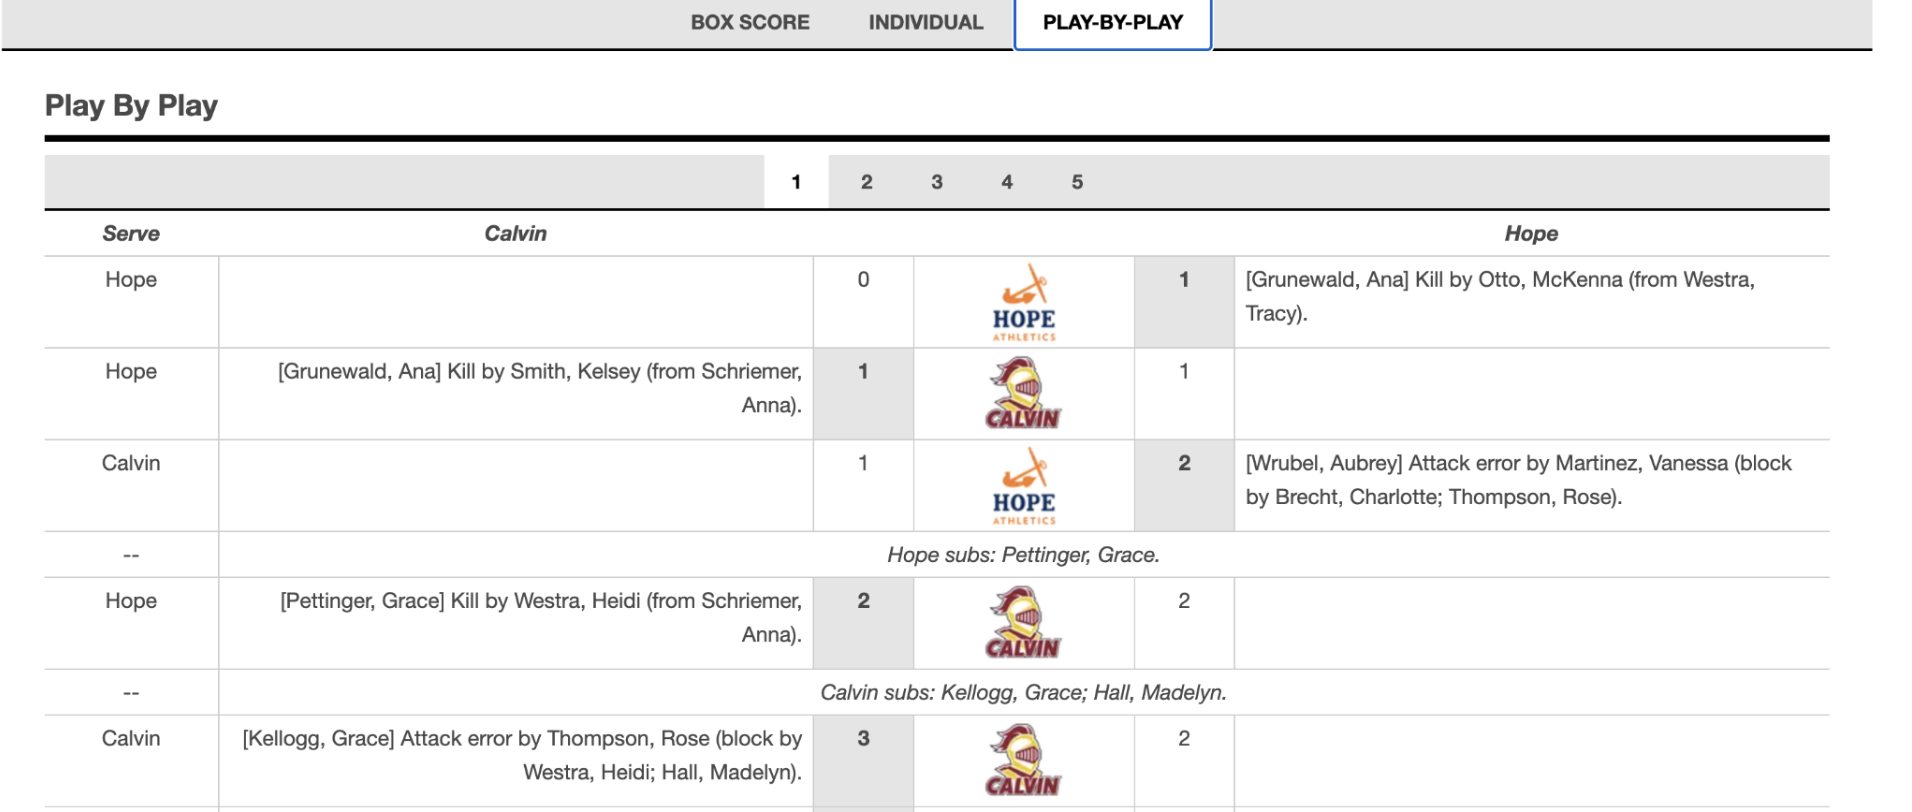
\includegraphics[width=\pw, height=\ph, keepaspectratio]{images/pbp.png}}%
        {\tikz\node[draw=black!30, fill=black!5, minimum width=\pw, minimum height=\ph,
           font=\tiny\ttfamily, text=black!50]{pbp.png};}};
\draw[flow] ($(pbp.south)+(0,-0.12)$) -- ($(out.north)+(0,0.12)$);
\draw[flow] ($(kdeduration.east)+(0.95,0)$) -- ($(out.west |- kdeduration.east)+(-0.2,0)$);
\end{scope}
% hand-off (b) -> (c): the frame-by-frame data feed the per-huddle measurements
\def\laneC{-17.7}
\draw[handoff] ($(maplbl.south)+(0,-0.1)$) -- (maplbl.south |- 0,\laneC) -- (8.15,\laneC) -- (8.15,-18.15);
\node[hchip] at ($(8.15,\laneC)!0.5!(maplbl.south |- 0,\laneC)$) {\figNRaw\ $\to$ \figNKept\ team-huddles after filtering};
%
\end{tikzpicture}%
}
\caption{\textbf{(a)} We collected 32 NCAA Division III women’s volleyball games (2019–2025) from YouTube. We prompted an MLLM (gemini-3.1-pro-preview) to identify start and stop times for every post-point huddle, and a human reviewed each answer using a labeling tool. Games had three to five sets, each averaging 45 huddles, except the fifth, which averaged 25. \textbf{(b)} We fed each huddle clip through a two-step video segmentation model (SAM 3): the first step identified the court to build homography for camera distortion correction, and the second detected and tracked on-court players at 30 fps, giving each player’s position in every frame. \textbf{(c)} After removing tracking errors and non-huddle moments, we track the diameter of the smallest circle enclosing a team’s players (red circle, bird’s-eye view) through the break, giving one curve per huddle. We then derive closeness (smallest distance), latency (time to come together), and duration (time staying together). Kernel density plots show each feature’s distribution across all huddles.}
%
\label{fig:pipeline}
\end{figure}
% ===== END PIPELINE FIGURE =====

\subsection{Data Extraction}
Our data consisted of multiple teams and multiple schools. Some schools have multiple games per year, and some have multiple games across years. A single team is defined as the same school and year. Additionally, the games span different importance levels, including non-conference games, regular-season conference games, post-season conference games, and NCAA post-season games. The 32 games yielded 5,571 post-point huddle moments, which amounted to 11,142 individual huddles, since every post-point huddle moment includes two unique huddles, one for each team. Also, we obtained in-game performance metrics for each game from the home team's play-by-play website. This performance data gave us information related to which team won which point, who scored and contributed to the point, and whether or not an error occurred. 

We selected games filmed with a tactical side-angle camera that did not change angle during the huddles. A human identified the start and stop times of each game to shorten the video before cutting the individual huddles. Once we identified the smaller chunks of the full game video, we used Gemini 3.1 Pro Preview to identify the start and stop times of each huddle throughout the entire game \citep{gemini31pro2026}. We defined the start of a huddle as when the point ended, the ball hit the ground, and players began moving toward one another. We defined the end of the huddle as the time at which both teams had dispersed from their huddle. A single start-and-stop time encompassed both teams' huddle. A single set, averaging around 45 huddles, cost \$2.72, or \$0.060 per huddle. After Gemini identified the timestamps of each huddle, a human used a labeling tool to modify, add, or delete the huddles. The human-verification process was essential, as mistakes in the number or length of huddles would negatively impact subsequent analysis. After each huddle was cleanly cut and included, we saved the raw individual clips as mp4 files. 


\subsection{Model}
To model the players' locations, which we later used to calculate team-level features, we used the vision-language model SAM3. SAM3 is a unified model that can detect, segment, and track objects throughout an entire video \citep{sam3_2025}. SAM3 is particularly useful for its open-vocabulary detection embedding. We used SAM3 for two phases in our pipeline–court detection and player detection.

\subsubsection{Court Detection}
First, we used SAM3 to identify the volleyball court, specifically the lines and corners. This was necessary because camera angles distort depth perception. We prompted the model with ``white court lines," but this prompt could generalize to ``$<$color$>$ court lines". The segmented lines, along with additional calculus to identify the line type (end line versus attack line) and an extension mechanism to find intersection points, helped us identify the necessary corner points. We used these corner points to calculate the homography matrix, given the true corner locations of a simple 18m x 9m volleyball court. We applied the homography matrix to the player locations to obtain more accurate 2D locations \citep{hartley2004multiple}. 

\begin{figure}[htbp]
  \centering
  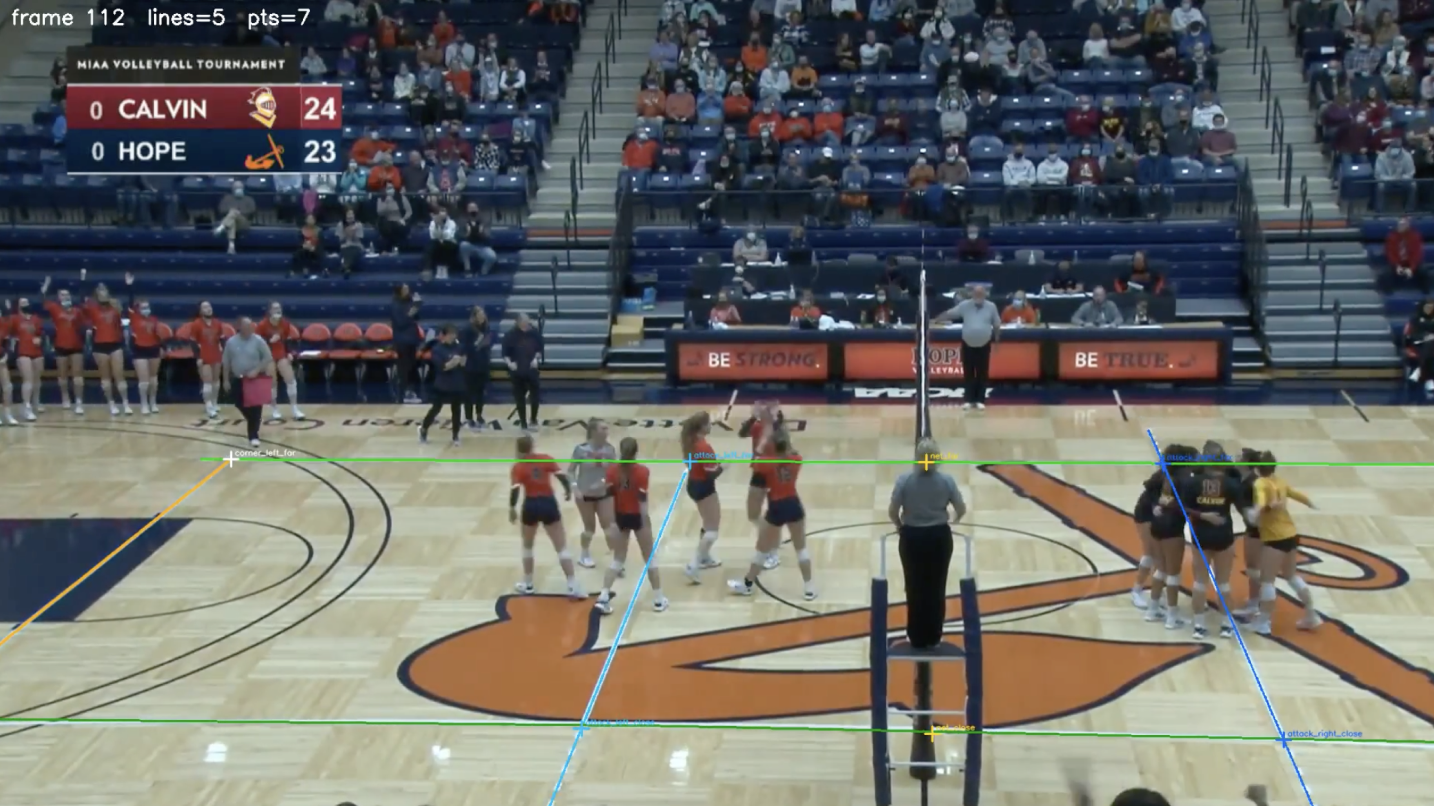
\includegraphics[width=0.5\linewidth]{white_court.png}
  \caption{Colored lines detected and segmented by SAM3, and the white points at the corners created by extended segments and grouped angle values to correctly classify corners to their correct location.}
  \label{fig:white_court}
\end{figure}


\subsubsection{Player Detection}
Our second use case with SAM3 was for detecting and tracking the players on the court. First, we prompted the model with ``female volleyball player playing." This prompt was necessary to filter out coaches, refs, and fans that the model could mistakenly pick up with a more vague prompt. Second, we filtered the allowed player locations to the detected court from the court detection phase. This helped avoid tracking players that may be standing on the sideline but who were not playing in the game. We were able to include players who may have run off the court to chase an in-play ball and came into frame later in the video by re-injecting the prompt in frames 30 and 45. 

Lastly, volleyball huddles are subject to occlusion. Players on the opposite side of the huddle from the camera are likely occluded by teammates' bodies. However, since the players' location is the bottom of their segmented box, and for most players that is the ground, we applied extrapolation logic to occluded players to estimate their location on the court. First, we identified all full masks throughout the huddle video and binned them by y-value to evenly cover each depth value. We then linearly regressed on all non-noisy segments based on height, defined as the player's head (y\_max) minus the player's feet (y\_min). We applied the slope and intercept to all players deemed occluded. These were players whose mask bottom overlapped with another player’s mask and whose mask was less than 90\% of the expected height. We also added a condition that occluded masks must be square-shaped rather than rectangular (this helped avoid incorrectly extrapolating diving players). 

\begin{figure}[H]
  \centering
  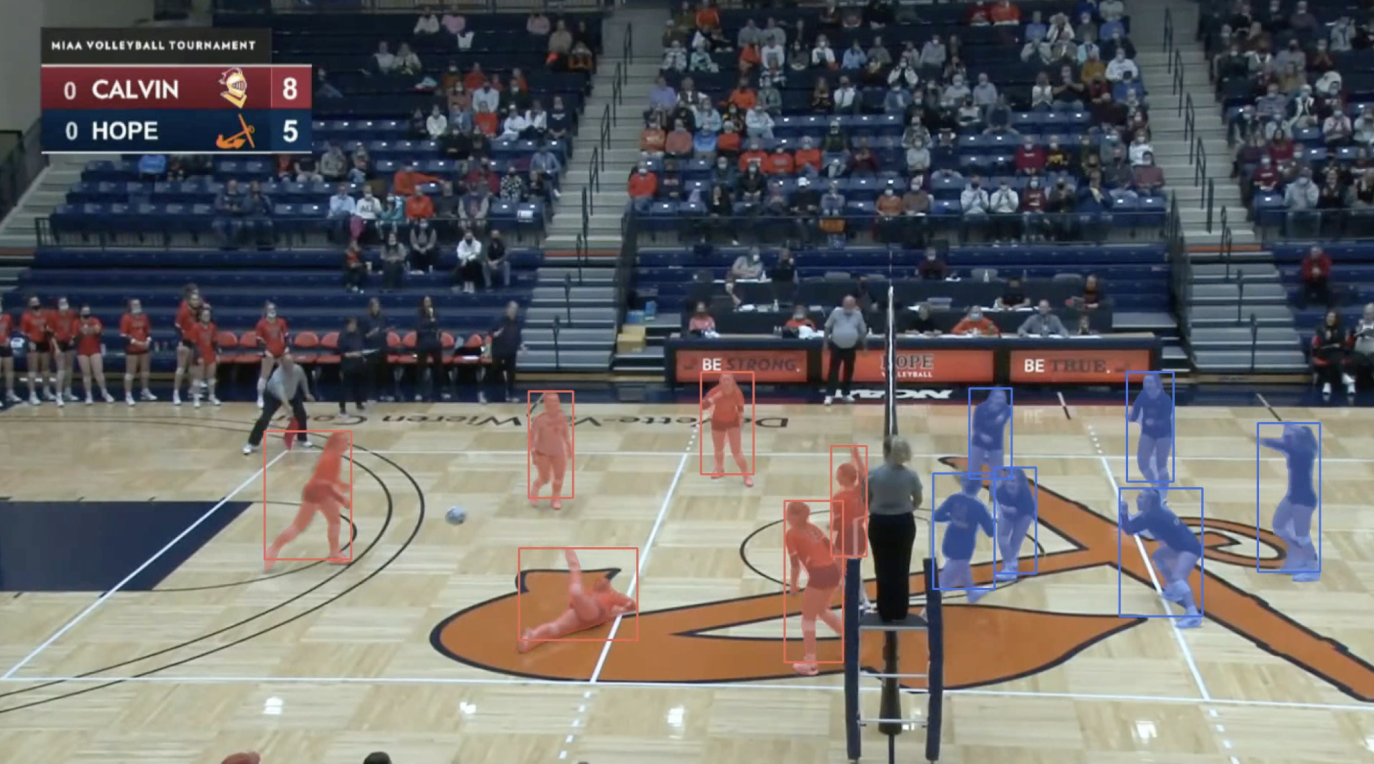
\includegraphics[width=0.5\linewidth]{player_track.png}
  \caption{Players detected through the extrapolation and on-court logic. We classified teams as right or left based on their position relative to the court center.}
  \label{fig:white_court}
\end{figure}

\subsubsection{Huddle Properties}
Once we obtained all correctly located player masks, we calculated team-level features from all individual locations. The three main features we identified were \textit{huddle closeness}, \textit{huddle duration}, \textit{huddle latency}. Since the huddle embodies the entire transition phase where interpersonal processes and, by its reciprocal nature, emergent states are quantifiable, we believed that measuring the ``degree" of the action would be more powerful than just the binary value of whether or not the huddle occurred. For this reason, we chose these three properties to measure the huddle as a whole. We defined huddle closeness as the closest the team got during their huddle. We calculated it as the enclosing circle diameter (in ft) anchored on the minimum-gyration value via Welzl's algorithm \citep{welzl1991smallest}. We defined huddle duration as the amount of time the team stays close in their huddle. We calculated it as the time (in seconds) a team stays within 1.5 times the dataset median radius. Lastly, we defined huddle latency as the time it took the team to get to their eventual closest huddle value. We calculated it as the elapsed time from the team's first tracked spread size to their eventual closest value, controlled for starting position size. Together, these properties tell us how quickly a team comes together, how long they stay together, and how close they get after a point. 

\begin{table}[htbp]
  \centering
  \small
  \renewcommand{\arraystretch}{1.3}
  \begin{tabular}{@{}l >{\raggedright\arraybackslash}p{0.22\linewidth}
                      >{\raggedright\arraybackslash}p{0.42\linewidth} c@{}}
    \hline
    \textbf{Feature} & \textbf{What it captures} & \textbf{How it is computed} & \textbf{Unit} \\
    \hline
    Closeness & How tight teammates huddle
      & Minimum enclosed-circle diameter over the huddle using Welzl's algorithm
      & ft \\
    Latency & How quickly the team comes together
      & Time from the first tracked frame to the frame at closeness value, controlled for starting position
      & s \\
    Duration & How long the team stays together
      & Time the team's enclosed circle stays within $1.5\times$ the data set median radius
      & s \\
    \hline
  \end{tabular}
  \caption{Huddle features computed from the smallest enclosing circle of a team's on-court players.}
  \label{tab:huddle_features}
\end{table}


Also, we identified non-huddles as huddles where closeness never reached 5ft and three or more players were 2.5ft from the center. Together, these conditions helped identify huddles that never fully formed. Non-huddles can happen for many reasons, ranging from a true non-huddle to players arguing with the ref and not coming together. We found no clear pattern between point outcome and non-huddling: 3.03\% of potential huddle opportunities were not huddles after a win, and 4.00\% after a loss.

\subsubsection{Outcome Data}
In addition to huddle properties, we obtained outcome-specific data from each game's play-by-play site. The play-by-play data has extensive information on how a point was scored, by whom, and what other players were involved–either if they errored or contributed by assisting. This information allows us to automate the relationship between a huddle and the point outcome before and after it. We could also quickly calculate momentum or losing-streak values the same way by cumulating momentum scores as outcomes \{-1, +1\} over the span of a set. 

Additionally, this data allowed us to create features related to how teams score their points–whether multiple players score or if it is the same couple of players every play. We also created Shannon entropy approximations to understand play type and player impact by measuring how diverse a team's scoring is \citep{shannon1948}. Lastly, we created features related to re-involvement, which let us track how players show up after making errors.

We also encountered some modeling risks. We identified tracking noise in our model based on the number of players detected throughout the video or an irregular huddle shape. Additionally, during labeling, some huddles were filmed at the wrong angle or missed entirely, so we cut clips with fewer than 10 frames and flagged them. We filtered out huddles identified as tracking noise, camera-angle issues, or non-huddles, resulting in the 10,362 clean huddles for our analysis. 
\end{document}
